\section{Réalisation (partie pratique)}
\label{sec:realisation}

\subsection{Objectif de la campagne de mesures}
L'objectif est de vérifier expérimentalement les modèles théoriques de la section précédente :
\begin{itemize}
\item résistance du primaire par les méthodes 2 fils et 4 fils ;
\item caractéristiques DC \(B=f(I)\) pour \(x=\SI{2}{mm}\) et \(x=\SI{3}{mm}\) ;
\item comportement AC du primaire et du secondaire à \(\SI{35}{Hz}\) ;
\item estimation de \(L_{12}\) et observation de la boucle \(B\)-\(H\) en mode \(x-y\).
\end{itemize}

\subsection{Appareillage utilisé}

\begin{table}[H]
\centering
\caption{Instruments de mesure et numéros d'inventaire HEIG-VD}
\begin{tabular}{llll}
\toprule
Appareil & Modèle & S/N & Inventaire \\
\midrule
Oscilloscope        & Tektronix DPO2014B & ---          & 11E 894-13 \\
Multimètre (4 fils) & HP 34181A          & US36056912   & 01E-1031   \\
Alimentation DC     & GW INSTEK PPE-3323 & ---          & 35E 037-07 \\
Teslamètre          & Hirst GM08         & GM08-1039    & PT9985     \\
\bottomrule
\end{tabular}
\label{tab:appareils}
\end{table}

\subsection{Résistance du primaire (4.1)}

\subsubsection{Protocole}
La résistance \(R_1\) est mesurée au multimètre selon deux méthodes :
\begin{itemize}
\item \textbf{2 fils} : la résistance inclut les fils de connexion ; valeur surestimée.
\item \textbf{4 fils} (méthode Kelvin) : le courant et la tension sont mesurés séparément ; la résistance des fils est éliminée.
\end{itemize}
Si la température \(T\neq\SI{20}{\degreeCelsius}\), on corrige :
\[
R_1(20)=\frac{R_1(T)}{1+\alpha(T-20)}.
\]

\subsubsection{Résultats}

\begin{table}[H]
\centering
\caption{Mesures de résistance du primaire}
\begin{tabular}{lcccc}
\toprule
Méthode & \(R_1\) mesuré [\si{\ohm}] & Température [\si{\degreeCelsius}] & \(R_1(20)\) [\si{\ohm}] & Écart à \SI{6.65}{\ohm} [\%] \\
\midrule
2 fils & 6.190 & 20 & 6.190 & $-6.9$ \\
4 fils & 6.164 & 20 & 6.164 & $-7.3$ \\
\bottomrule
\end{tabular}
\label{tab:R1_mes}
\end{table}

\subsubsection{Commentaire}
La mesure 4 fils (\SI{6.164}{\ohm}) est plus fiable car elle s'affranchit de la résistance des fils de connexion. La différence entre les deux méthodes, \(\Delta R=\SI{0.026}{\ohm}\), correspond à environ \SI{75}{cm} de fils de connexion (résistance de fil : \(\approx\SI{0.035}{\ohm/m}\)).

L'écart à la valeur théorique \(R_{1,\mathrm{th}}=\SI{6.65}{\ohm}\) est de \(-7.3\,\%\). Cet écart s'explique par :
\begin{itemize}
\item la tolérance sur le diamètre du fil \(\varnothing\SI{0.4}{mm}\) (\(\pm 2\,\%\) typique) ;
\item la longueur réelle de fil légèrement inférieure à l'estimation par le périmètre moyen ;
\item la résistivité du cuivre réel (\(\rho_{20}=\SI{1.72e-8}{\ohm.m}\) nominal, mais dépend de la pureté).
\end{itemize}

\subsection{Mesure de l'induction \texorpdfstring{\(B=f(I)\)}{B=f(I)} en DC (4.2)}

\subsubsection{Protocole}
Une sonde de Hall (teslamètre) est placée dans un entrefer latéral. Une cale étalon règle l'entrefer ; elle reste en place dans les deux entrefers pendant toute la mesure. Le courant DC est balayé de \(\SI{0}{A}\) à \(\SI{0.6}{A}\) par pas de \(\SI{0.1}{A}\).

\subsubsection{Résultats}

\begin{table}[H]
\centering
\caption{Relevés \(B=f(I)\) — branche montante}
\begin{tabular}{ccccccccc}
\toprule
\(I\) [A] & 0.0 & 0.1 & 0.2 & 0.3 & 0.4 & 0.5 & 0.6 \\
\midrule
\(B\) [mT], \(x=\SI{2}{mm}\) & 0 & 10.35 & 19.14 & 27.79 & 36.7 & 45.6 & 54.3 \\
\(B\) [mT], \(x=\SI{3}{mm}\) & 0 & 6.61  & 11.8  & 17.3  & 22.8  & 28.1 & 33.7 \\
\bottomrule
\end{tabular}
\label{tab:Bmes_mont}
\end{table}


\begin{figure}[H]
\centering
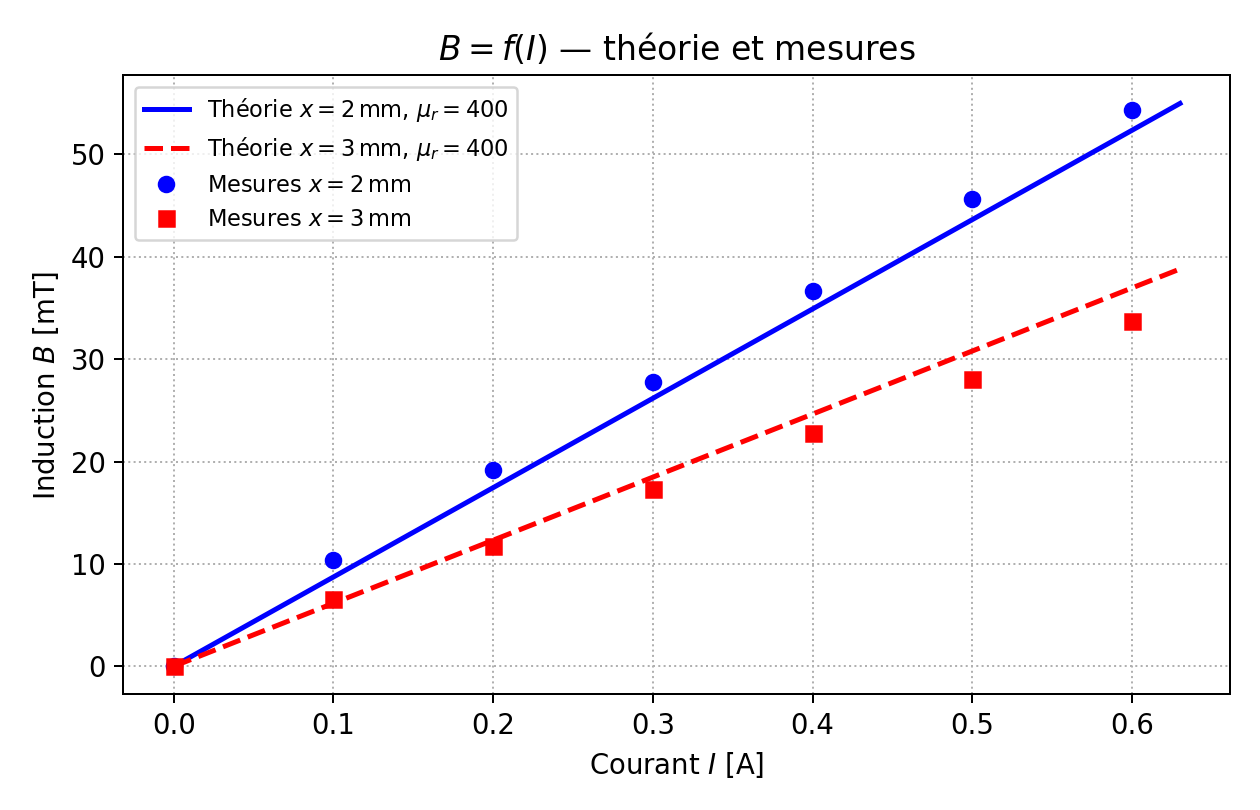
\includegraphics[width=0.85\textwidth]{images/BfI_comp.png}
\caption{Comparaison théorie / mesures pour \(B=f(I)\)}
\label{fig:BfI_comp}
\end{figure}

\subsubsection{Commentaire}
\begin{itemize}
\item Les deux courbes \(B=f(I)\) sont quasi linéaires sur la plage \(0\)–\(\SI{0.6}{A}\), ce qui confirme l'absence de saturation marquée dans cet intervalle.
\item Pour un même courant, \(B\) est plus élevé pour \(x=\SI{2}{mm}\) que pour \(x=\SI{3}{mm}\), conformément à la théorie (réluctance d'entrefer plus faible).
\item Le rapport des pentes mesurées \(k_{2\mathrm{mm}}/k_{3\mathrm{mm}}\approx88.1/54.2\approx1.63\) est proche du rapport théorique \(3.4/2.4=1.42\) (\(\mu_r=400\), \(\lambda=0.4\,\mathrm{mm}\)).
\item L'accord quantitatif théorie/mesure est de l'ordre de \(\pm 5\,\%\) à \(\pm 9\,\%\) (voir tableau de synthèse), ce qui valide le modèle à 3 entrefers.
\end{itemize}

\subsection{Mesures AC primaire-secondaire à \SI{35}{Hz} (4.3)}

\subsubsection{Protocole}
Régler \(f=\SI{35}{Hz}\), viser \(\hat{I}_1\approx\SI{300}{mA}\) crête via l'amplificateur linéaire. Mesures pour \(x=0\) puis \(x=\SI{2}{mm}\).

Grandeurs relevées : \(\hat{U}_1\), \(\hat{I}_1\), déphasage \(\varphi(i_1,u_1)\).

\begin{table}[H]
\centering
\caption{Mesures AC de référence à \SI{35}{Hz}}
\begin{tabular}{lccc}
\toprule
Entrefer & \(\hat{U}_1\) [V] & \(\hat{I}_1\) [A] & \(\varphi(i_1,u_1)\) [\(^\circ\)] \\
\midrule
\(x=0\)              & 20.8 & 0.276 & 73.3 \\
\(x=\SI{2}{mm}\)     & 2.95  & 0.300 & 49.5 \\
\bottomrule
\end{tabular}
\label{tab:AC_ref}
\end{table}

\begin{figure}[H]
\centering
\begin{minipage}[t]{0.48\textwidth}
\centering
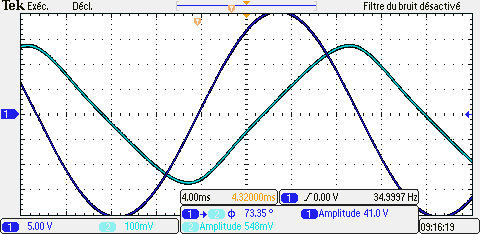
\includegraphics[width=\textwidth]{images/TEK00000.PNG}
\caption*{\(x=0\,\mathrm{mm}\) — \(\varphi=73.35°\), \(f=35{,}0\,\mathrm{Hz}\)}
\end{minipage}\hfill
\begin{minipage}[t]{0.48\textwidth}
\centering
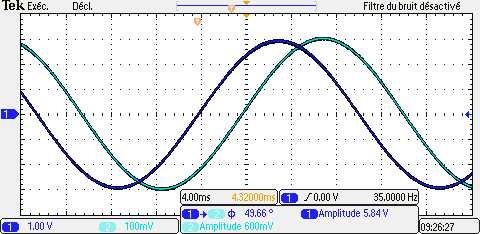
\includegraphics[width=\textwidth]{images/TEK00001.PNG}
\caption*{\(x=\SI{2}{mm}\) — \(\varphi=43.66°\), \(f=35{,}0\,\mathrm{Hz}\)}
\end{minipage}
\caption{Captures oscilloscope — \(U_1\) (CH1) et \(I_1\) (CH2) à \SI{35}{Hz}}
\label{fig:oscillo_AC}
\end{figure}

\subsubsection{Commentaire}
La tension \(U_1\) chute de \(\SI{20.8}{V}\) (à \(x=0\)) à \(\SI{2.95}{V}\) (à \(x=\SI{2}{mm}\)) pour un courant quasi-identique, ce qui reflète la forte diminution de \(L_{11}\) avec l'entrefer. À \(x=0\), l'amplificateur atteignait sa limite de tension (générateur bloquant). On peut estimer l'inductance et les paramètres du circuit à partir de ces mesures :

\[
|Z_1|=\frac{\hat{U}_1}{\hat{I}_1}, \quad
\omega L_{11}=|Z_1|\sin\varphi, \quad
R_{1,\mathrm{eff}}=|Z_1|\cos\varphi.
\]

\begin{table}[H]
\centering
\caption{Paramètres estimés à \SI{35}{Hz}}
\begin{tabular}{lcccc}
\toprule
Entrefer & \(|Z_1|\) [\si{\ohm}] & \(\omega L_{11}\) [\si{\ohm}] & \(L_{11}\) [mH] & \(R_{1,\mathrm{eff}}\) [\si{\ohm}] \\
\midrule
\(x=0\)          & 75.4 & 72.2 & 328 & 21.7 \\
\(x=\SI{2}{mm}\) & 9.83 & 7.47 & 33.9 & 6.39 \\
\bottomrule
\end{tabular}
\label{tab:AC_params}
\end{table}

À \(x=\SI{2}{mm}\), la résistance effective (\SI{6.39}{\ohm}) est proche de \(R_1=\SI{6.16}{\ohm}\), ce qui indique que les pertes fer sont faibles à grand entrefer. À \(x=0\), la résistance effective est nettement plus élevée (\SI{21.7}{\ohm}), révélant des pertes par hystérèse et courants de Foucault significatifs lorsque le flux est intense.

Quand l'entrefer augmente, l'inductance \(L_{11}\) diminue (réluctance croissante), ce qui :
\begin{itemize}
\item réduit \(U_1\) pour un même courant \(I_1\) (impédance plus faible) ;
\item réduit le déphasage \(\varphi\) (comportement plus résistif).
\end{itemize}

\subsection{Intégrateur à ampli-op et diagramme de Bode (4.3.2)}

Le montage intégrateur (annexe, \(R_9=R_{11}=\SI{10}{k\ohm}\), \(R_{10}=\SI{100}{k\ohm}\), \(C=\SI{1}{\mu F}\)) a pour fonction de transfert :
\[
H(j\omega)=\frac{U_{\mathrm{out}}}{U_{\mathrm{in}}}=-\frac{R_{10}}{R_9}\cdot\frac{1}{1+j\omega R_{10}C}.
\]
Fréquences caractéristiques :
\[
f_c=\frac{1}{2\pi R_{10}C}=\frac{1}{2\pi\times10^5\times10^{-6}}\approx\SI{1.59}{Hz},
\qquad
f_{0\mathrm{dB}}=\frac{1}{2\pi R_9 C}=\frac{1}{2\pi\times10^4\times10^{-6}}\approx\SI{15.9}{Hz}.
\]
À \(\SI{35}{Hz}\gg f_c\), le montage est en régime quasi-intégrateur pur : \(|H|\approx R_{10}/(R_9\cdot\omega R_{10}C)=1/(\omega R_9 C)\).

\begin{figure}[H]
\centering

\includegraphics[width=0.85\textwidth]{images/bode_dernier_circuit.png}
\caption{Diagramme de Bode de l'intégrateur
(\(R_9{=}R_{11}{=}\SI{10}{k\ohm}\), \(R_{10}{=}\SI{100}{k\ohm}\), \(C{=}\SI{1}{\mu F}\))}
\label{fig:bode_integ}
\end{figure}

\subsection{Diagramme B-H en mode \texorpdfstring{\(x-y\)}{x-y} et estimation de \texorpdfstring{\(L_{12}\)}{L12} (4.3.3 / 4.3.4)}

Sur l'oscilloscope en mode \(x-y\) :
\begin{itemize}
\item axe \(x\) : tension aux bornes d'une résistance shunt proportionnelle à \(i_1(t)\) ;
\item axe \(y\) : sortie de l'intégrateur proportionnelle à \(\int u_2\,dt \propto \Phi(t) \propto B(t)\).
\end{itemize}
Le tracé obtenu est une image de la boucle \(B\)-\(H\) à facteur d'échelle près.

\paragraph{Variation avec l'entrefer.}
En augmentant \(x\), la boucle s'allonge horizontalement (courant plus grand pour un même flux) et s'amincit (pertes hystérétiques plus faibles). La pente de la droite centrale est proportionnelle à \(L_{12}\).

\paragraph{Estimation de \(L_{12}\).}
En régime sinusoïdal, la tension induite au secondaire est \(U_2=j\omega L_{12}I_1\), d'où :
\[
L_{12}=\frac{|U_2|}{\omega\,|I_1|}.
\]

\begin{figure}[H]
\centering
\begin{minipage}[t]{0.48\textwidth}
\centering
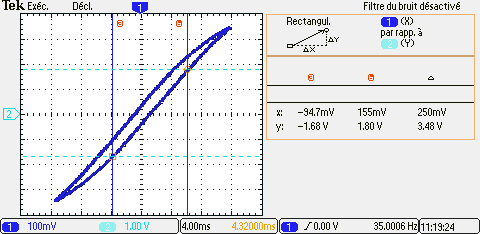
\includegraphics[width=\textwidth]{images/TEK00005.PNG}
\caption*{\(x=0\,\mathrm{mm}\) — \(\Delta x=250\,\mathrm{mV}\), \(\Delta y=3{,}48\,\mathrm{V}\)}
\end{minipage}\hfill
\begin{minipage}[t]{0.48\textwidth}
\centering
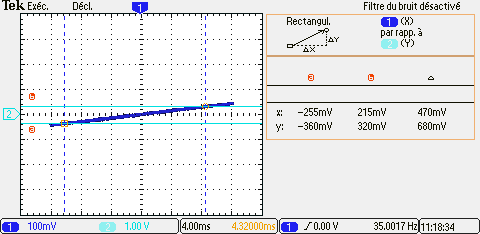
\includegraphics[width=\textwidth]{images/TEK00004.PNG}
\caption*{\(x=\SI{2}{mm}\) — \(\Delta x=470\,\mathrm{mV}\), \(\Delta y=680\,\mathrm{mV}\)}
\end{minipage}
\caption{Boucles \(B\)-\(H\) en mode \(x\)-\(y\) avec curseurs \(\Delta\) (mesure de \(L_{12}\))}
\label{fig:BH_xy}
\end{figure}

\begin{table}[H]
\centering
\caption{Estimation de \(L_{12}\) à partir de la mesure AC}
\begin{tabular}{lccc}
\toprule
Entrefer & \(L_{12}\) mesuré [mH] & \(L_{12}\) théorique [mH] & Écart [\%] \\
\midrule
\(x=0\,\mathrm{mm}\)$^*$ & 139 & 34.6 & $+302$ \\
\(x=\SI{2}{mm}\)          & 14.5 & 5.8  & $+150$ \\
\bottomrule
\end{tabular}
\label{tab:L12_mes}
\end{table}

\subsection{Synthèse — comparaison théorie / mesure}

\begin{table}[H]
\centering
\caption{Tableau de synthèse}
\begin{tabular}{p{5.2cm}p{2.8cm}p{2.8cm}p{2.8cm}}
\toprule
Grandeur & Théorie & Mesure & Écart [\%] \\
\midrule
\(R_1(20)\) [\si{\ohm}]                                & 6.65   & 6.164  & $-7.3$ \\
\(B\) à \(I=\SI{0.5}{A}\), \(x=\SI{2}{mm}\) [mT]      & 43.6   & 45.6   & $+4.6$ \\
\(B\) à \(I=\SI{0.5}{A}\), \(x=\SI{3}{mm}\) [mT]      & 30.8   & 28.1   & $-8.7$ \\
\(L_{11}\) à \(x=\SI{2}{mm}\) (AC) [mH]               & 14.4   & 33.9   & $+135$ \\
\(L_{12}\) à \(x=0\,\mathrm{mm}\)$^*$ [mH]             & 34.6   & 139    & $+302$ \\
\(L_{12}\) à \(x=\SI{2}{mm}\) [mH]                    & 5.8    & 14.5   & $+150$ \\
\bottomrule
\end{tabular}
\label{tab:comparaison}
\end{table}
